\documentclass[11pt,a4paper]{article}
\usepackage[T1]{fontenc}\usepackage[utf8]{inputenc}\usepackage{lmodern,amsmath,amssymb,graphicx,booktabs,array,microtype,float,placeins}
\usepackage[margin=25mm]{geometry}\usepackage[hidelinks]{hyperref}\usepackage{fancyhdr,caption}
\pagestyle{fancy}\fancyhf{}\fancyhead[L]{Solar Hydrogen Production and Storage}\fancyfoot[C]{\thepage}\setlength{\headheight}{14pt}
\setlength{\parindent}{0pt}\setlength{\parskip}{6pt}\captionsetup{font=small,labelfont=bf}
\begin{document}
\begin{titlepage}\centering\vspace*{25mm}
{\huge\bfseries Solar Hydrogen Production and Storage\par}\vspace{7mm}
{\Large Annual TRNSYS Simulation for Phoenix Arizona\par}\vspace{8mm}{\large Homework 2\par}\vspace{20mm}
{\Large Pouya Asghari\par}\vspace{10mm}
Renewable Energies Course\par Adviser: Dr. Pouria Ahmadi\par
\vfill School of Mechanical Engineering\par College of Engineering, University of Tehran\par
Original report date: 1404.09.06 (Iranian calendar)\par
\end{titlepage}
\section*{Editorial note}
This edition converts the supplied English Word report into LaTeX. The original narrative, numerical claims, equations, tables, references, and figures are retained, with duplicate Word caption text removed. The student number is omitted. The original TRNSYS files are supplied unchanged alongside the report. The simulation has not been rerun during this conversion.

Some source claims are inconsistent with mass conservation or with the saved model. In particular, compression does not increase hydrogen mass production, and the post-compression mass conversion requires verification of the component's volume-reference conditions. The separate editorial appendix documents these issues; the historical values in the body should not be treated as validated design results.
\begingroup\small\setlength{\parskip}{0pt}\tableofcontents\endgroup\clearpage


\FloatBarrier
\section{Abstract}

This study examines the performance of a solar-powered hydrogen production and storage system modeled under the climate conditions of Phoenix, Arizona using TRNSYS. The goal is to design and evaluate an integrated setup in which photovoltaic power drives an alkaline electrolyzer capable of producing approximately 5 kg of hydrogen per day, followed by compression to 200 bar for storage. The system is developed by updating PV module properties according to the VSUN450-144BMH catalog and constructing a dynamic TRNSYS model that includes solar power generation, electrolysis, hydrogen compression, and storage processes. TRNSYS serves as the main simulation platform, using Arizona weather data, component models, and operational control strategies to simulate system behavior throughout an entire year. The results identify the necessary series--parallel configuration of solar panels, the hourly and monthly hydrogen production rates, the hydrogen consumption profile after compression, and the electrolyzer polarization curve. These outcomes demonstrate the potential for reliable hydrogen generation when coupling high solar availability in Phoenix with electrolytic production and high-pressure storage.

\section*{Nomenclature}
\begin{tabular}{ll}\toprule Symbol & Meaning\\\midrule
$A$ & Area [m$^2$]\\$\rho$ & Density [kg/m$^3$]\\$V$ & Voltage [V]\\$I$ & Current [A]\\PEM & Proton exchange membrane\\PV & Photovoltaic\\AEL & Alkaline electrolyzer\\HP & Hydrogen production\\HC & Hydrogen consumption\\\bottomrule\end{tabular}

\FloatBarrier
\section{Introduction}

The transition toward low-carbon energy systems has increased global interest in renewable resources capable of providing reliable and sustainable power. Among the various renewable options, solar energy has become one of the most widely adopted due to its abundance, accessibility, and direct conversion into electricity through photovoltaic technologies. Photovoltaic (PV) systems operate by transforming sunlight into electrical power using semiconductor materials, allowing clean electricity generation with minimal environmental impact. Despite these advantages, solar energy remains inherently intermittent, fluctuating with daily and seasonal variations in irradiance. This intermittency limits direct use in many applications and highlights the need for effective energy-storage solutions.

Hydrogen has emerged as a promising energy carrier for storing surplus renewable electricity. It can be produced through electrolysis, a process in which electrical energy splits water into hydrogen and oxygen. Several electrolyzer technologies exist, including alkaline, proton exchange membrane (PEM), and solid oxide electrolyzers, each offering different efficiencies, operating conditions, and system requirements. Alkaline electrolyzers, in particular, are mature, commercially available, and well-suited for integration with solar power due to their stability and relatively low operating cost. Once produced, hydrogen can be compressed, stored, and later used in various sectors such as transportation, industrial processes, and electricity generation, making it a flexible medium for long-term energy storage.

The integration of photovoltaic systems with electrolyzers and hydrogen storage has gained attention as a complete pathway for converting solar energy into a storable and dispatchable fuel. Modeling such systems enables evaluation of their performance under realistic climatic and operational conditions. Simulation tools such as TRNSYS provide a platform for studying the dynamic interactions between components, assessing energy flows, and optimizing system configurations over extended periods.

The present study focuses on developing and analyzing a solar-powered hydrogen production and storage system under the environmental conditions of Phoenix, Arizona. A PV array based on the VSUN450-144BMH module is coupled with an alkaline electrolyzer, a compressor, and a high-pressure storage tank. The objective of the work is to determine the PV configuration required to produce approximately 5 kg of hydrogen per day, simulate the system using TRNSYS, and evaluate hydrogen production rates, post-compression consumption, and electrolyzer performance over a full year.

\FloatBarrier
\section{System Description}

The system operates by converting solar radiation into electrical power through a photovoltaic array, which supplies the energy required to drive an alkaline electrolyzer that splits water into hydrogen and oxygen. The produced hydrogen then passes through a compressor that raises its pressure to 200 bar before entering a high-pressure storage tank for long-term containment. Throughout the cycle, TRNSYS models the dynamic interaction between components, including solar input, electrical generation, electrolysis behavior, and compression stages. The schematic of the system shown in Fig. 1 represents a sequential flow beginning with the PV panels, followed by the electrolyzer, compressor, and final storage unit, illustrating how solar energy is transformed step-by-step into stored hydrogen fuel.

\begin{figure}[H]\centering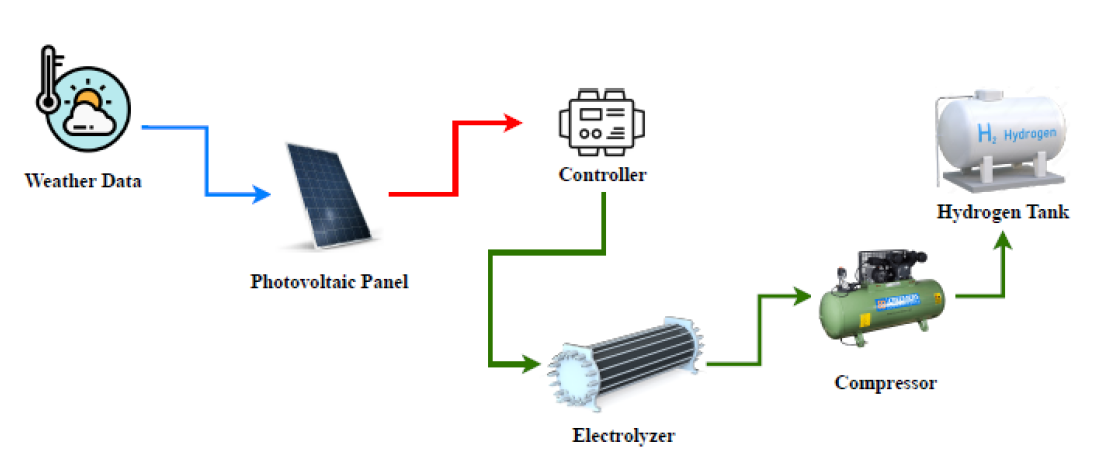
\includegraphics[width=0.96\linewidth,height=0.48\textheight,keepaspectratio]{figures/rId6.png}\caption{Schematic of the solar hydrogen system.}\end{figure}

\FloatBarrier
\section{Modeling in TRNSYS}

The TRNSYS model is used to analyze the transient behavior of the photovoltaic system and the alkaline electrolyzer, with the goal of determining the number of PV panels required for producing 5 kg of hydrogen per day. In the subsequent stage, the generated hydrogen is compressed using a high-pressure compressor and stored in a dedicated tank, after which the daily and hourly hydrogen consumption rates are evaluated and plotted.

\FloatBarrier
\section{Part A PV and Electrolyzer}

This part focuses on developing a dynamic TRNSYS model that links the photovoltaic array to an alkaline electrolyzer for hydrogen production. This part evaluates the number of panels required and simulates the hourly and monthly hydrogen generation over a full year.

\subsection{Design}

A PV panel (Type 103-a module) is first added to the TRNSYS model, and its parameters are updated based on the specifications provided in the VSUN450-144BMH catalog.

\begin{table}[H]\centering\caption{PV module catalog properties as transcribed in the source.}
\begin{tabular}{lll}\toprule Parameter & Value & Unit\\\midrule
$P_{\max}$ & 450 & W\\$V_{oc}$ & 49.4 & V\\$I_{sc}$ & 11.52 & A\\$V_{mpp}$ & 41.2 & V\\$I_{mpp}$ & 10.93 & A\\NOCT & 45 & $^\circ$C\\Voltage temperature coefficient & -0.27 & V/K\\Current temperature coefficient & +0.048 & A/K\\\bottomrule\end{tabular}\end{table}

The initial configuration assumes one module in series and ten modules in parallel. The latitude of Phoenix, approximately 34 degrees, is applied as the array slope in the PV settings. All remaining environmental inputs are connected to the TMY2 weather data file. A controller is then added to verify whether the input voltage supplied to the electrolyzer meets the required threshold. The idling power is set to 1700 W, and a Type 175a power-conditioning module is included to regulate power flow. An alkaline electrolyzer is added to the system, with the PV power output routed through the controller and the power set point connected to the conditioning module. The output current of the conditioning module is linked to the electrolyzer current input, while the electrolyzer voltage is linked back to the conditioning module output voltage. This closed loop ensures convergence of values over time and functions as a feedback mechanism. Finally, the hydrogen production rate is extracted from the electrolyzer, noted to be in units of m\textsuperscript{3}/hr, and converted to kg/hr using an equation module. The operating pressure of the Alkaline Electrolyzer (AEL) is 7 bar, with an assumed operating temperature of 50 degrees Celsius. Under these conditions, the density of hydrogen is 0.5282 kg/m\textsuperscript{3} [1]. The hydrogen production rate in kg/hr is calculated by multiplying this density by the volumetric hydrogen production rate (HP). An integrator component is then used to determine the total mass of hydrogen produced. The daily average hydrogen production is obtained by dividing the integrator's annual total output by 365. Similarly, the monthly average is calculated by dividing the annual total by 12. The resulting daily average values are compared against the target production rate of 5 kg/day, as specified in the assignment requirements.

Through iterative adjustment of the series and parallel panel configurations, where the number of parallel panels proved more influential, a final configuration of 30 panels in series and 7 in parallel was determined. This configuration yields a daily hydrogen production rate of 4.91 kg/day, as recorded by the printer component, which closely approximates the target value of 5 kg/day.

\begin{figure}[H]\centering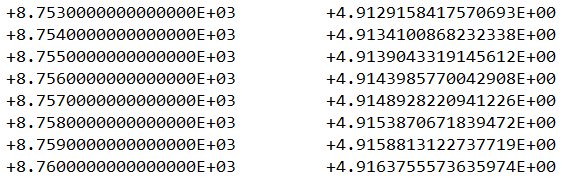
\includegraphics[width=0.96\linewidth,height=0.48\textheight,keepaspectratio]{figures/rId7.png}\caption{Reported daily hydrogen production indicator.}\end{figure}

With the simulation now finalized, the hourly and monthly hydrogen production rates for the system can be exported.

\begin{figure}[H]\centering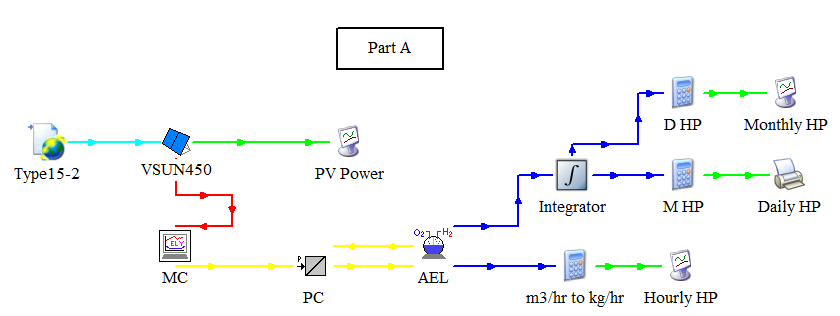
\includegraphics[width=0.96\linewidth,height=0.48\textheight,keepaspectratio]{figures/rId8.png}\caption{TRNSYS schematic for Part A.}\end{figure}

Furthermore, with the number of panels determined, the power output of the PV array can be plotted as shown in Fig. 4.

\begin{figure}[H]\centering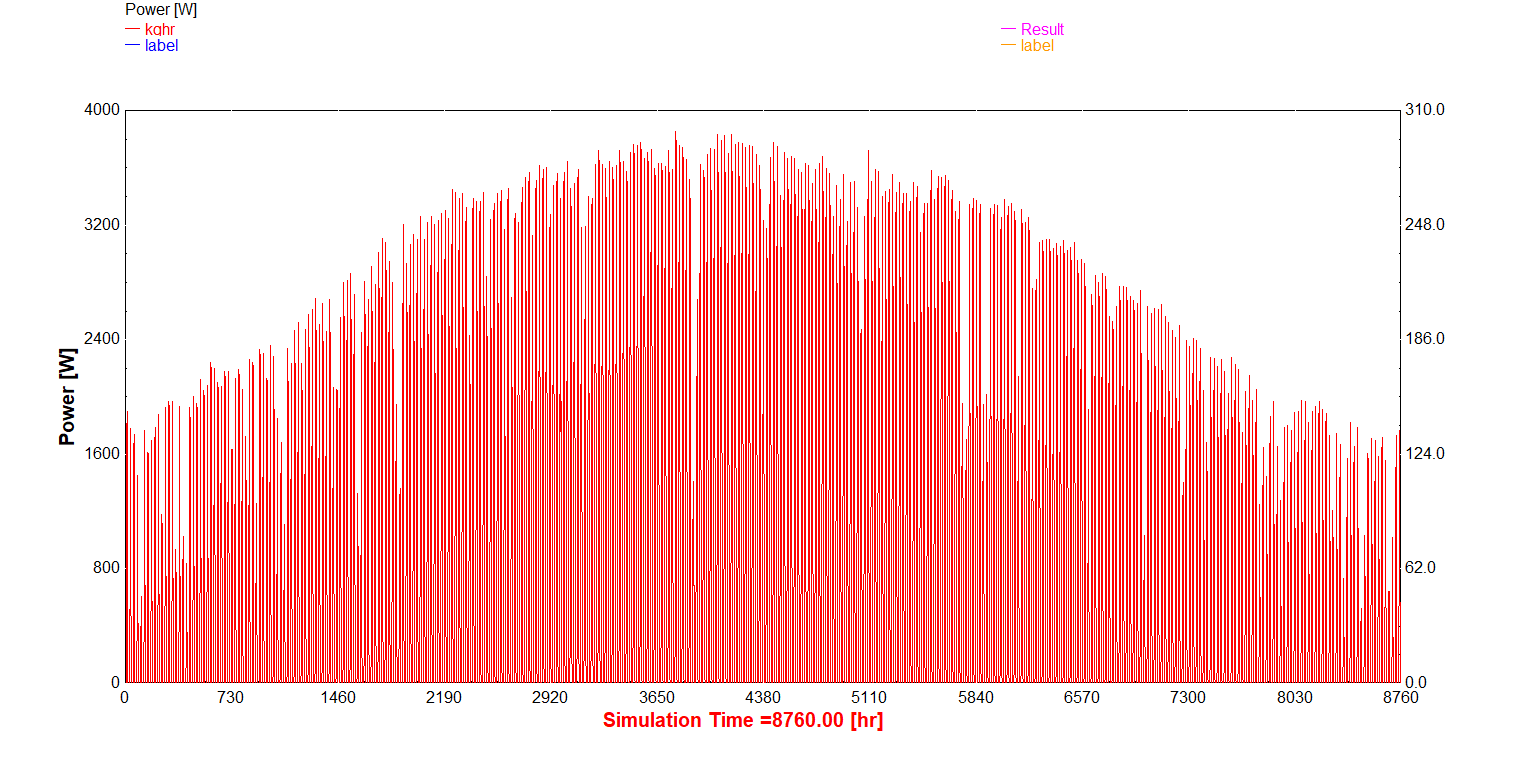
\includegraphics[width=0.96\linewidth,height=0.48\textheight,keepaspectratio]{figures/rId9.png}\caption{PV power over one year in Phoenix Arizona.}\end{figure}

The hourly hydrogen production rate can also be visualized by applying Equation (1) and plotting the resulting values.

\begin{equation}\dot m_{\mathrm{H_2}}=\dot V_{\mathrm{H_2}}\rho=HP\times0.5282\quad[\mathrm{kg/h}].\end{equation}

\begin{figure}[H]\centering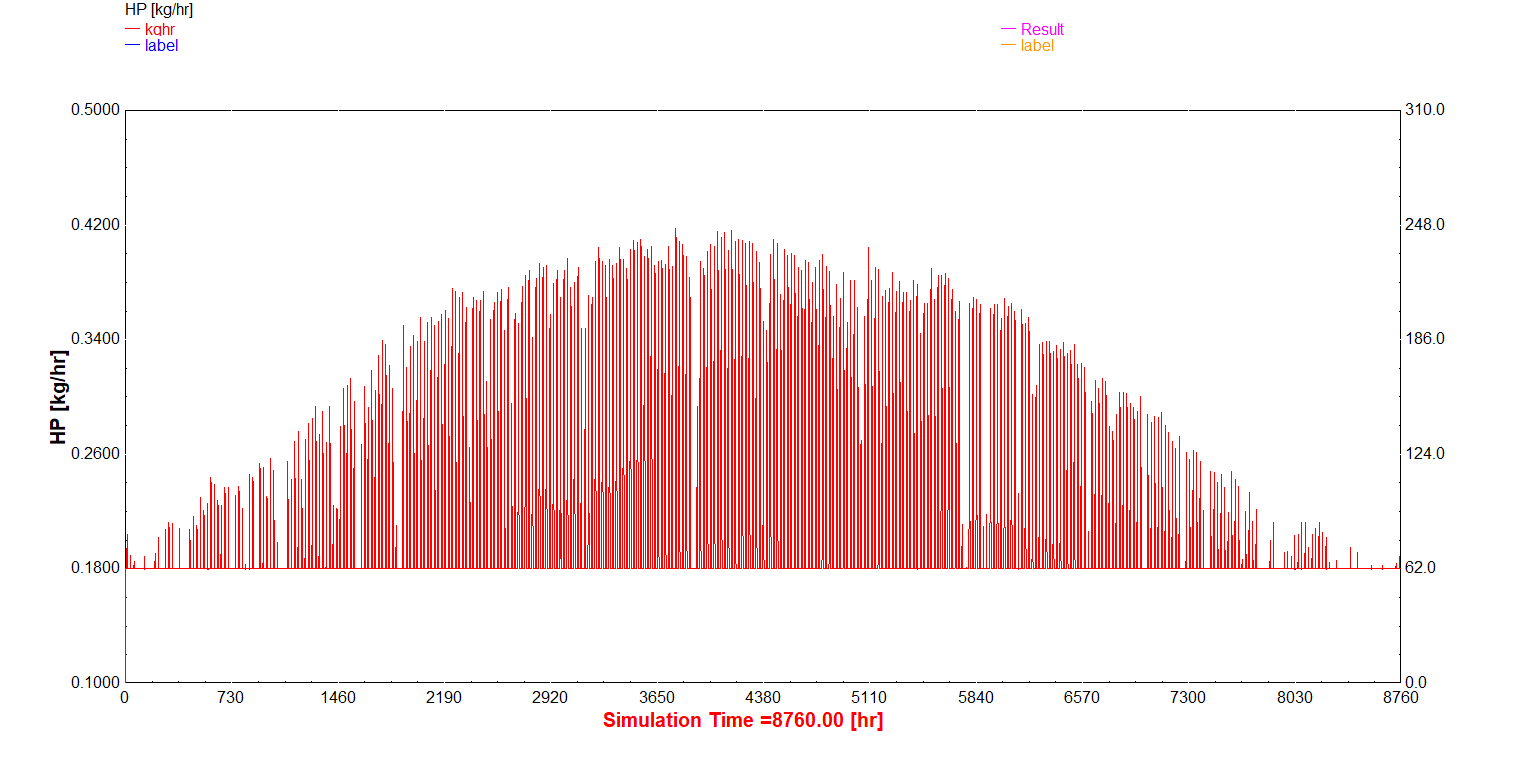
\includegraphics[width=0.96\linewidth,height=0.48\textheight,keepaspectratio]{figures/rId10.png}\caption{Reported hourly hydrogen production.}\end{figure}

The monthly hydrogen production is calculated by integrating the total production and dividing the result by 12. Consequently, Equation (1) can be extended to formulate Equation (2) for plotting the monthly production. As shown in Fig. 6, the final value of the plot reaches 150 kg/month, which is equivalent to the target production rate of 5 kg/day.

\begin{equation}HP\rho\frac{8760}{12}=HP\times0.5282\times\frac{8760}{12}=HP\times385.586\quad[\mathrm{kg/month}].\end{equation}

\begin{figure}[H]\centering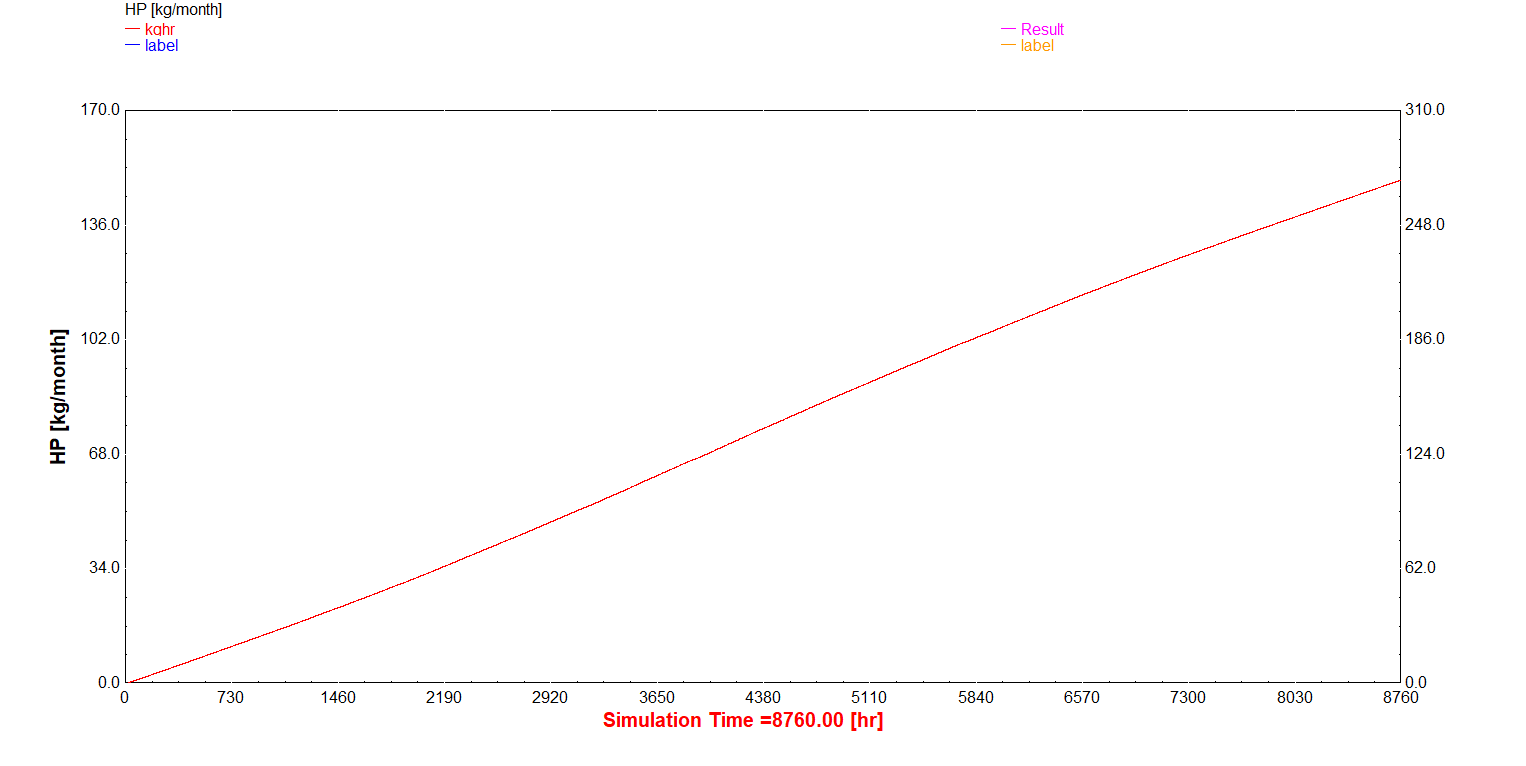
\includegraphics[width=0.96\linewidth,height=0.48\textheight,keepaspectratio]{figures/rId11.png}\caption{Reported monthly hydrogen production indicator.}\end{figure}

\FloatBarrier
\section{Part B Compression and Storage}

This part involves compressing the produced hydrogen to a storage pressure of 200 bar using a compressor and storing it in a designated tank. The analysis requires plotting the hourly and daily hydrogen consumption rates following the pressure increase, as well as the polarization curve for the electrolyzer.

\subsection{Design}

The system configuration preceding the electrolyzer remains identical to the previous model. The modeling is extended by integrating a compressor and a storage tank into the system. The storage tank is connected to a controller to establish a feedback loop based on the storage pressure. This control logic is implemented such that when the pressure within the tank surpasses 90 percent of its maximum allowable pressure of 350 bar, the controller sends a signal to cut power to the electrolyzer. Production remains halted until the tank pressure decreases to 70 percent of the maximum, at which point the controller sends another signal to restore power and recommence hydrogen production.

The compressor functions to increase the pressure of the hydrogen produced by the Alkaline Electrolyzer (AEL) from its initial 7 bar to a final 200 bar. This pressurization facilitates large-scale storage and concurrently increases the hydrogen production rate. The storage tank has a defined volume of 370 m\textsuperscript{3}. The key output for analysis is the output flow rate from the compressor. This flow rate data is then processed similarly to the previous analysis to plot the hourly and daily hydrogen consumption rates. Due to the pressure increase to 200 bar, the density of hydrogen changes; at 200 bar and a temperature of 80 degrees Celsius, the density is 13.6297 kg/m\textsuperscript{3} [1]. For calculating the daily average consumption value, the total integrated mass from the simulation is divided by 365, as opposed to the division by 12 that was used for deriving the monthly production values in Equation (2).

\begin{equation}HP\rho\frac{8760}{365}=HP\times13.6297\times\frac{8760}{365}=HP\times327.1128\quad[\mathrm{kg/day}].\end{equation}

\begin{figure}[H]\centering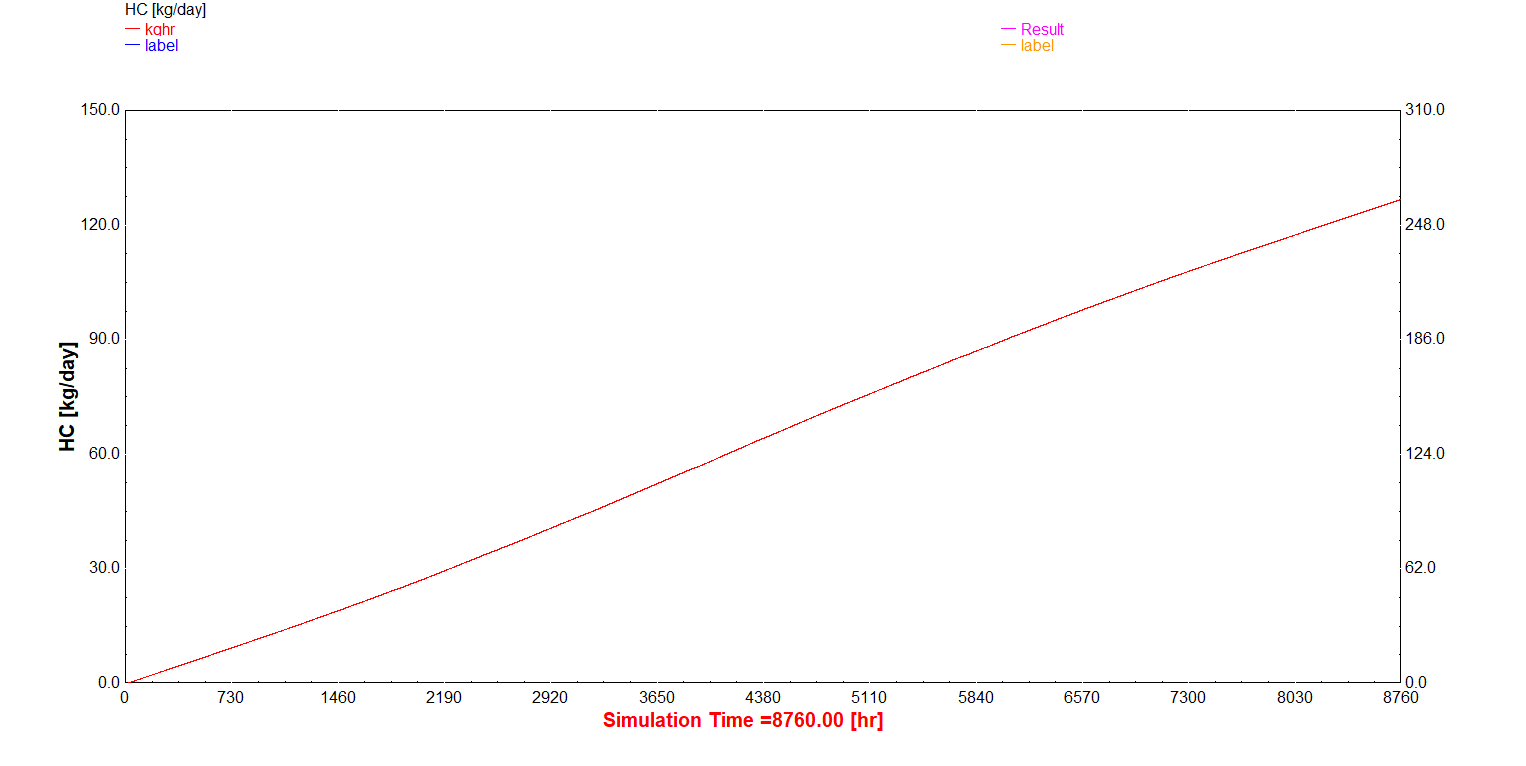
\includegraphics[width=0.96\linewidth,height=0.48\textheight,keepaspectratio]{figures/rId12.png}\caption{Reported daily hydrogen consumption indicator.}\end{figure}

As shown in Fig. 7, the daily hydrogen mass flow rate after the compressor reaches 127 kg. This value is 24 times greater than the flow rate observed prior to compression, indicating a significant increase in the effective production rate. The compressor outlet flow rate can subsequently be converted into units of kg/hr for plotting the hourly consumption.

\begin{figure}[H]\centering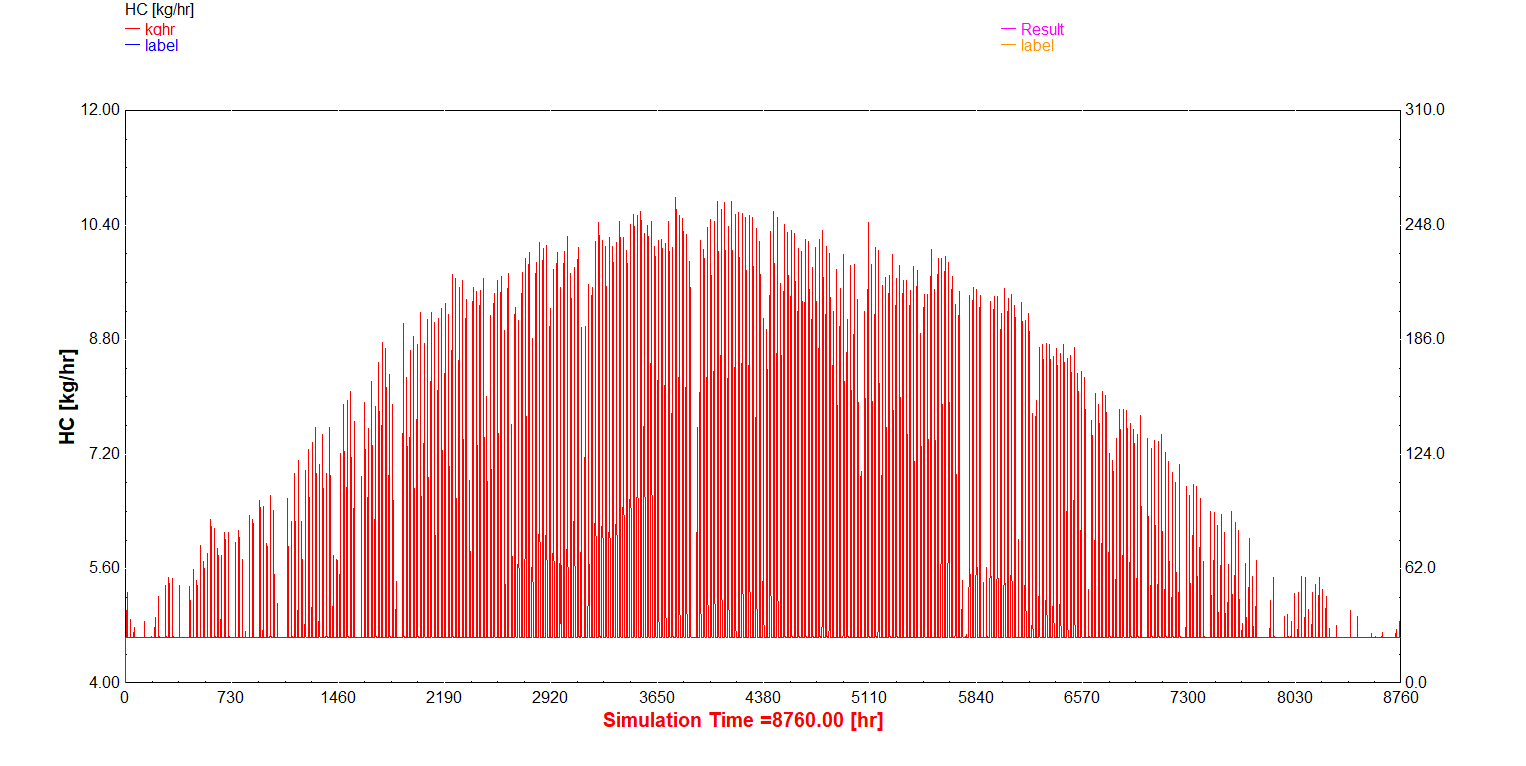
\includegraphics[width=0.96\linewidth,height=0.48\textheight,keepaspectratio]{figures/rId13.png}\caption{Reported hourly hydrogen consumption indicator.}\end{figure}

The finalized system configuration is presented in Fig. 9.

\begin{figure}[H]\centering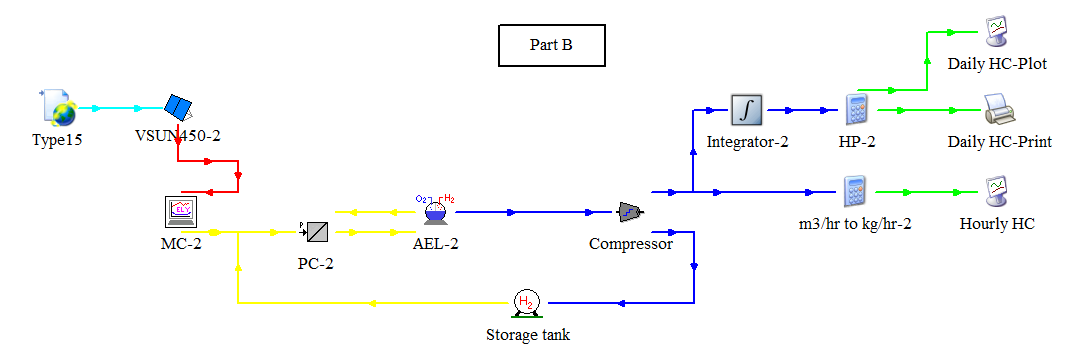
\includegraphics[width=0.96\linewidth,height=0.48\textheight,keepaspectratio]{figures/rId14.png}\caption{TRNSYS schematic for Part B.}\end{figure}

The polarization curve for the Alkaline Electrolyzer (AEL) is generated by using a time-dependent function as the input current. This input is scaled by a factor of 10 and supplied to the AEL component. The corresponding output voltage from the AEL is then plotted against the input current using an online plotter, which requires the use of an equation module to define the relationship.

\begin{equation}\mathrm{current}=\mathrm{time}\times0.1.\end{equation}

\begin{figure}[H]\centering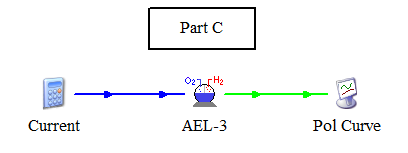
\includegraphics[width=0.96\linewidth,height=0.48\textheight,keepaspectratio]{figures/rId15.png}\caption{TRNSYS schematic used to generate the polarization curve.}\end{figure}

As observed in Fig. 11, the TRNSYS simulation successfully models the activation and ohmic polarization regions of the electrolyzer but does not accurately represent the concentration polarization, which is characterized by a sharp voltage increase at high current densities. The absence of this feature in the model is likely because the selected alkaline electrolyzer (AEL) operates well within its safe operational limits, specifically below the maximum current density threshold where mass transport limitations become significant.

Concentration resistance, or mass transport overpotential, becomes prominent when the rate of reactant supply (water) or product removal (hydrogen and oxygen bubbles) cannot keep pace with the electrochemical reaction rate at the electrode surface. This typically occurs at very high current densities, near the operational limit of the cell. The implemented model parameters, particularly the maximum allowable current density of 1000 mA/cm\textsuperscript{2}, may define a safe operating window where the reaction kinetics and ionic conductivity are the dominant factors, and the diffusion limitations are negligible. Consequently, the modeled polarization curve exhibits a predominantly linear behavior in the high-current region instead of the characteristic exponential rise, indicating that the system is not being driven into a mass-transport-limited regime under the simulated conditions.

\begin{figure}[H]\centering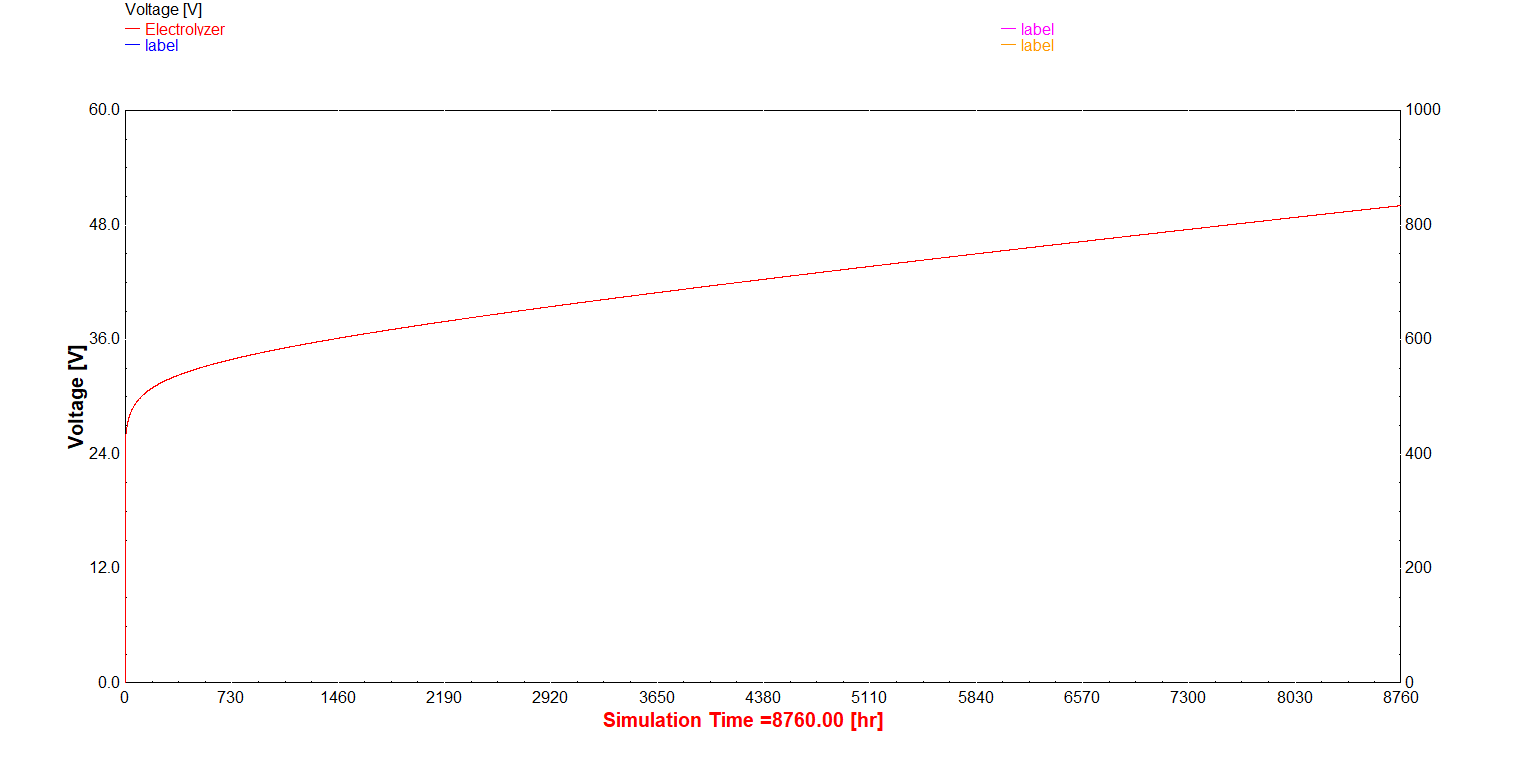
\includegraphics[width=0.96\linewidth,height=0.48\textheight,keepaspectratio]{figures/rId16.png}\caption{Electrolyzer polarization curve.}\end{figure}

\FloatBarrier
\section{Results and Discussion}

The simulation of the solar-powered hydrogen production and storage system was successfully executed in TRNSYS for the climate of Phoenix, Arizona. The system was designed, sized, and its dynamic performance was analyzed over a full year, with key results presented for hydrogen production, storage, and electrolyzer efficiency.

\subsection{PV System Sizing and Hydrogen Production}

The primary objective was to determine the photovoltaic (PV) array configuration required to achieve an average daily hydrogen production of 5 kg. Through an iterative process, it was found that the number of parallel strings had a more significant impact on the total current and, consequently, the hydrogen output than the number of series-connected panels. The optimal configuration was determined to be 30 panels in series and 7 strings in parallel, yielding a total of 210 panels of the VSUN450-144BMH model.

This configuration produced a daily average hydrogen output of 4.91 kg/day, as recorded by the integrator and printer components in TRNSYS. This value is within 2\% of the target 5 kg/day, confirming the configuration's suitability. The PV power output, shown in Fig. 4, exhibits the expected diurnal and seasonal variations characteristic of solar energy in Phoenix. The corresponding hourly hydrogen production rate, calculated using Equation (1) with a hydrogen density of 0.5282 kg/m\textsuperscript{3} at the electrolyzer's operating conditions (7 bar, 50$^\circ$C), reflects this variable power input.

The monthly hydrogen production, derived by integrating the total annual production and dividing by 12 (Equation (2)), consistently averaged 150 kg/month (Fig. 6). This result directly correlates to the 5 kg/day target and validates the system's ability to meet the annual production goal.

\subsection{System Performance with Compression and Storage}

The integration of the compressor and a high-pressure storage tank introduced critical dynamics for managing the stored hydrogen. The controller successfully maintained the tank pressure within the predefined safety limits of 70\% to 90\% of the maximum 350 bar by cycling the electrolyzer's power, preventing over-pressurization.

The compressor increased the hydrogen pressure from 7 bar to 200 bar, significantly increasing the gas density to 13.6297 kg/m\textsuperscript{3} (at 80$^\circ$C). Analysis of the compressor's output flow rate revealed a substantial daily hydrogen mass flow of 127 kg/day (Fig. 7). This value, which is 24 times greater than the flow rate measured before compression, does not represent a physical increase in production but rather reflects the increased mass of gas per unit volume at the higher pressure. This demonstrates the system's effectiveness in converting a volumetric flow of low-density hydrogen into a dense, storable energy carrier. The hourly consumption rate (Fig. 8) further illustrates the intermittent operation dictated by the controller and the variable solar resource.

\subsection{Electrolyzer Polarization Curve Analysis}

The polarization curve for the Alkaline Electrolyzer (AEL), generated by plotting the output voltage against a scaled time-dependent input current, is presented in Fig. 11. The model accurately captures the activation and ohmic polarization regions, which are characteristic of the initial voltage requirement to initiate the reaction and the linear voltage increase due to ionic resistance in the electrolyte, respectively.

However, the characteristic sharp voltage increase associated with concentration polarization at very high current densities is not observed. This absence is attributed to the defined operational limits of the model. The maximum allowable current density of 1000 mA/cm\textsuperscript{2} likely establishes a safe operating window where the system does not reach the mass-transport-limited regime. In this regime, the supply of reactants (water) to the electrodes or the removal of product gases (H\textsubscript{2} and O\textsubscript{2} bubbles) cannot keep pace with the reaction rate. Since the model operates within its designed limits, the diffusion limitations are negligible, and the polarization curve exhibits a predominantly linear behavior in the high-current region instead of the characteristic exponential rise. This behavior is physically consistent and indicates that the electrolyzer is modeled for stable, non-limiting operation under the simulated conditions.

\FloatBarrier
\section{References}

[1]Engineering 4E. (n.d.). H2 physical properties calculator. Retrieved December 1, 2024, from \url{https://www.engineering-4e.com/h2-physical-properties-calculator}

[2]National Oceanic and Atmospheric Administration. (n.d.). Solar resource data. National Centers for Environmental Information. Retrieved December 1, 2024, from \url{https://www.ncei.noaa.gov/products/solar-resource-data}

[3]National Renewable Energy Laboratory. (n.d.). System Advisor Model (SAM). U.S. Department of Energy. Retrieved December 1, 2024, from \url{https://sam.nrel.gov/}

[4]Shiva Kumar, S., \& Himabindu, V. (2019). Hydrogen production by PEM water electrolysis -- A review. Materials Science for Energy Technologies, 2(3), 442--454. \url{https://doi.org/10.1016/j.mset.2019.03.002}

[5]TRNSYS. (n.d.). Transient System Simulation Tool. Solar Energy Laboratory, University of Wisconsin-Madison. Retrieved December 1, 2024, from \url{https://www.trnsys.com/}

[6]U.S. Department of Energy. (n.d.). Hydrogen and fuel cell technologies office. Office of Energy Efficiency \& Renewable Energy. Retrieved December 1, 2024, from \url{https://www.energy.gov/eere/fuelcells/hydrogen-and-fuel-cell-technologies-office}

[7]Ahmadi P, (2025, October 5). Electrolyzer and fuel cell simulation in TRNSYS. Youtube. From \url{https://youtu.be/YdyufGXlPkE?si=dwf05GntS6_2rvpt}

\FloatBarrier
\section{Attachment}

\begin{figure}[H]\centering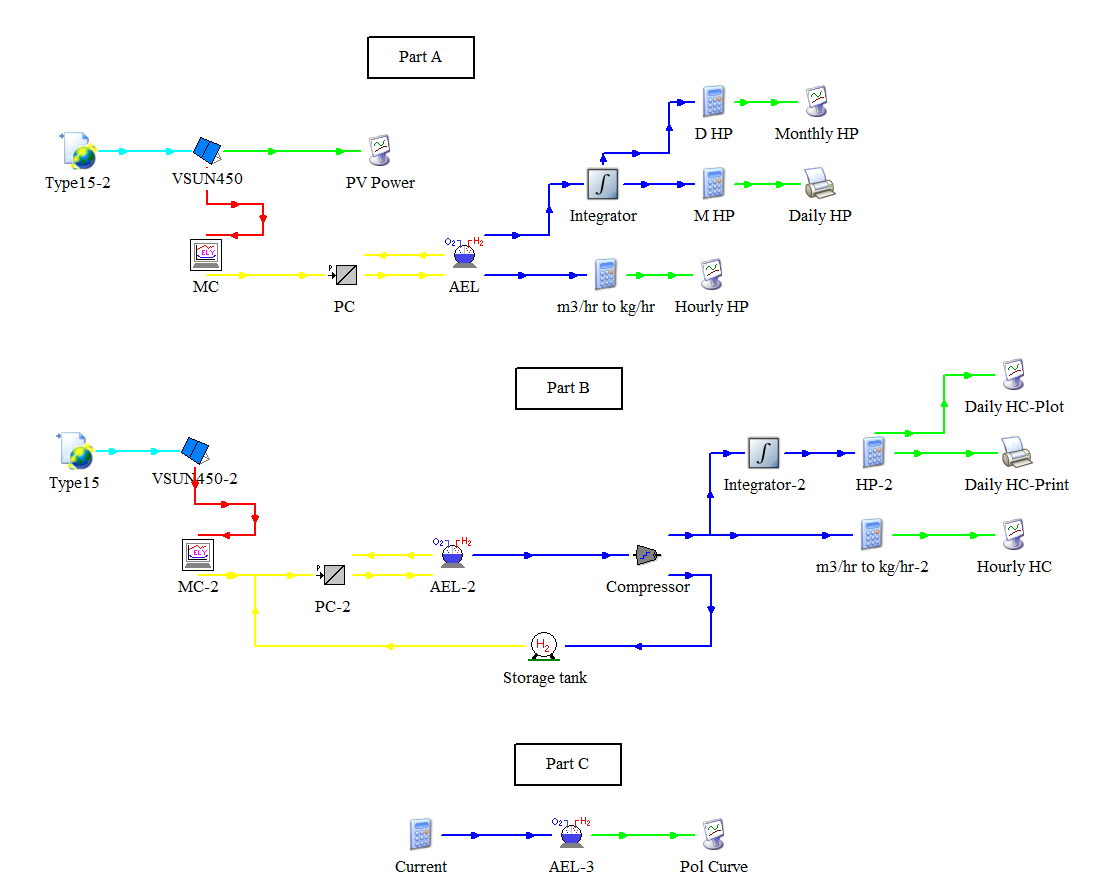
\includegraphics[width=0.96\linewidth,height=0.48\textheight,keepaspectratio]{figures/rId24.png}\caption{Full schematic of all TRNSYS simulation parts.}\end{figure}

\FloatBarrier\clearpage\appendix\section{Editorial Review of the Supplied Model}
This appendix was added during conversion. It does not change the original model or establish corrected simulation results.
\subsection{Saved outputs and array size}
The supplied \texttt{AEL\_Daily\_HP.out} ends at 8760 hours with a value of 4.9163755574. The file \texttt{HC\_daily.out} ends at the same time with 126.8602392138. The second value remains unvalidated as a physical hydrogen mass flow. The deck contains 30 modules in series and seven in parallel. At the stated 450 W module rating this is 210 modules and 94.5 kWp nameplate capacity, not a constant operating power.
\subsection{Compression and the volume reference basis}
The first conversion multiplies the AEL volume rate by 0.5282, whereas the compressor outlet rate is multiplied by 13.6297. The ratio of these densities is approximately 25.8, close to the ratio of the two saved indicators. This is a reason to investigate the volume reference basis, not proof of an increased mass production rate. The TRNSYS Type 160 and Type 167 documentation and proformas must establish whether the rates use actual or standard/reference volumes before the correct densities can be chosen. Steady compression of the same stream does not create hydrogen mass; any transient differences must be reconciled with accumulation, venting, or separate branches.
\subsection{Annual averaging and plots}
The deck integrates AEL flow and divides the cumulative result by 365 or 12. During the year these are cumulative totals divided by a fixed annual denominator. Only the final values represent the corresponding annual-average daily or monthly indicators under the selected conversion. They are not independent daily totals or twelve month-by-month production totals. The saved production indicator implies about 1794.48 kg/year and 149.54 kg per average month under that conversion. The body uses rounded values, including 4.91 kg/day and 150 kg/month.
\subsection{Storage pressure and controller settings}
Seventy and ninety percent of a 350 bar limit correspond to 245 and 315 bar, respectively. Both exceed the stated 200 bar compressor discharge pressure. The report does not demonstrate that this control band is attainable in the proposed configuration. The tank volume is stated and stored as 370 cubic meters; verify that this is the intended design scale. Pressure compatibility and the controller behavior need checking before asserting successful regulation.
\subsection{Component parameters and missing dependencies}
The deck refers to an absolute Windows path for the Phoenix TMY2 weather file and to \texttt{Type160-Electrolyzer.dat}. These external data files are not supplied. A compatible TRNSYS installation must provide the required component implementations, including the hydrogen components. The archived paths must be updated for a new machine.

The PV deck retains a cell count of 36 and module area of 0.89 square meters. These entries should be checked against the intended VSUN450-144BMH module. Temperature coefficients in the report and deck must also be checked against the catalog's unit convention, including whether the listed numbers are percentages or absolute coefficients. The module catalog is not included as a separate source file.
\subsection{Polarization and simulation warnings}
The narrative says the time input is scaled by ten, while Equation (4) uses a factor of 0.1. The log includes Type 160 low-voltage warnings for the polarization branch. The absence of a concentration-polarization upturn does not by itself establish that the real electrolyzer is operating safely; the chosen model may not represent that mechanism. Verify the component equations, units, parameter range, and current sweep before making that conclusion.
\subsection{Reproducibility status}
The supplied native project, deck, parameter file, log, listing, and two outputs are archived unchanged. The report has been compiled in LaTeX, but TRNSYS has not been executed during preparation. Additional separately stored code should be added with verified dependencies and run instructions. No missing weather data, component data, or corrected outputs have been invented.
\end{document}